\section{Study Design}
\label{sec:study_design}
To understand the motivations behind the creation and maintenance of variant forks we performed the following activities: (i) we designed the survey protocol, (ii) collected mainline--variant pairs and extracted the participants from the variant forks, and (iii) recruited the survey participants.

%we  and then . Next, we designed and developed a survey protocol that we used to recruit the participants.
 %The survey was run in April 2021 with the goal of understanding why developers create and maintain variant forks.

\subsection{Survey Protocol Design}
\label{sec:protocal}
Since our aim was to learn from a large number of participants, we opted to use surveys scale well as compared to interviews.
We used the knowledge gained from literature, especially the motivations we discussed in Section~\ref{sec:motivations} and designed a 12-question survey that would last at most 15 minutes. The 12 questions that were asked covered the three key research questions in this study of exploring motivation of creating and maintaining variant forks:

\begin{itemize}
\item Are there common developers between the variants and the mainline repositories? (RQ1)
\item What was the motivation behind creating\,/\,maintaining a variant fork? (RQ2)
\item Is there any interaction between the fork and the mainline repository during their co-evolution? (RQ3)
\end{itemize}

We designed the questions in such a way that the participants can choose the most appropriate reason from the provided options that best suits their motivations for forking. 8 of the 12 questions were closed-ended that included both multiple choice response questions and Likert-scale response questions to allow for more quantitative analysis. For 3 of the 8 closed-ended questions, we asked a total of 4 optional open-ended questions to provide respondents with an opportunity to share additional thoughts and feedback.

 %\ad{@John: I suggest to first explain how you designed the survey, then how you found/selected participants, then how you analyzed their answers.}


\subsection{Identifying variant projects and participants}
\label{sec:forks_and_participants}
To conduct the survey, we need developers involved in the creation and maintenance of variant projects and possibly potentially competing. We distinguish between two variant projects: (i) \emph{attached}--ones where the fork is still attached to the mainline (i.e., a direct traceability link between mainline and fork still exists that can be used for exchanging pull requests) and (ii) \emph{detached}--forks which are detached from the mainline (i.e., they were cloned and re-uploaded with no link exists between the mainline and the fork).
We relied on two data sources, \librariesio\footnote{https://libraries.io} and \gh.
For the \emph{attached}, we extracted some variant projects from \librariesio and the others from \gh.
\begin{itemize}
\item \librariesio: This contains metadata for distributed packages on various package registries; we extracted the metadata and filtered those projects that are forks of another one. We follow the variant identification method discussed in the previous studies of~\cite{businge:emse:2021,businge:benevol:2020}. We searched popular package registries of \texttt{npm}, \texttt{Go}, \texttt{Maven}, \texttt{Plpy}, \texttt{Packagist}.
As opposed to the previous studies, in this study our method of extracting variant projects was very restrictive since were only interested in those variants that are actively maintained in parallel with their mainline counterparts. We extracted variants where the mainline--variant pairs were created before \texttt{2019-04-01} and updated after \texttt{2020-04-01}.
At the end of this process, we \textit{had 227 mainline–variant project pairs}.

\item \gh: Since we wanted to increase our changes on the number of respondents in our survey, we also collected variant projects directly from \gh that were not among the 227 in the previous step. We searched popular mainline repositories (having $\geq 50$ forks) written in the 17 popular programming languages on \gh that include: JavaScript, Java, Go, Python, Ruby, C. For each the mainline, we extracted forks that were created before \texttt{2019-04-01} and updated after \texttt{2020-04-01}, having $\geq 10$ stargazers, having $\geq 10$ commits ahead of the mainline (unique commits), having $\geq 5$ closed pull requests, and where the fork and mainline differ in the contents of the \texttt{readme.md} file for description. We manually verify that the mainline and fork are indeed in two different projects by reading and comparing the contents of the \texttt{readme.md}. Using this process, \textit{we had an additional 225 mainline–variant project pairs}.
\end{itemize}

\nd \textbf{Identifying detached variant projects}. We used \gh search feature looking for repositories that are not referred as ``forks'' but that do contain ``fork of'' in their description and both the mainline and variant projects are actively maintained (i.e., were forked before \texttt{2019-04-01} and updated after \texttt{2020-04-01}; the mainline and variant have at least 100 commits after the fork date). We also manually verified that indeed the mainline and variant are indeed different projects being maintained in parallel by reading their \texttt{readme.md} pages. Using this process, \textit{we had an additional 40 mainline–variant project pairs}.
Overall from the three dataset extraction methods used, \textbf{we collected a total of 491 mainline--variant pairs}.

%\ad{I think there are too many (technical and practical) details in this section. This is likely to confuse the readers. I propose to focus on the main steps only, and to better motivate what we did. I propose the following outline: to conduct the survey, we need developers involved in the creation and maintenance of variant projects; to identify potentially competing variant projects; we distinguish between \emph{attached} and \emph{detached} projects; we relied on two data sources, namely Libraries.io and \gh; Libraries.io contains metadata for distributed packages on various package registries; we extracted the metadata and filtered those projects that are forks of another one using \gh API; we also used \gh search feature to find popular repositories and their forks; we manually filtered repositories corresponding to mainline projects and their variant projects; at the end of this step, we have XX \emph{attached} mainline-variant pairs; we also used \gh search feature looking for repositories that are not referred as ``forks'' but that do contain ``fork of'' in their description; at the end of this process, we have XX \emph{detached} mainline-variant pairs we manually checked; then we looked at the project history to find appropriate respondent candidates (how?); we contacted them, and got XX responses.}

% Like we discussed in Section~\ref{sec:intro} we stated that a variant fork of an mainline project is also a real product developed in parallel with the mainline, while providing a solution different from the mainline.
% We extract our dataset variant forks from two main sources: the first dataset is extracted from \librariesio\footnote{https://libraries.io} and the second dataset is extracted directly from \gh. We further classify the second dataset into two types: ones where the variant fork is still attached to the mainline (a direct traceability link between mainline and fork still exists that can be used for exchanging pull requests), and variant forks which are detached from the mainline (no direct traceablity link exists).

% \subsubsection{Libraries.io}
% \label{sec:library.io}
% We extracted the mainline--variant fork pairs from the most popular package managers for different programming language ecosystems that can be found on one central location \librariesio, which is a platform that periodically collects all data from different package managers, that include, \texttt{npm}, \texttt{Go}, \texttt{Maven}, \texttt{Plpy}, \texttt{Packagist}, etc. We extract the mainline--variant fork pairs from the latest \texttt{Libraries.io} data dump release 1.6.0 that was released on January 12, 2020. The meta-model for the data on the \texttt{Libraries.io} data dump can be found online.\footnote{https://libraries.io/data}
% We follow the following steps:

% \begin{enumerate}[label=\alph*.]
% \item  Using the package's field \texttt{Platform}, we filter out the packages that are distributed on popular package managers.

% \item Next, we use the field \texttt{Forkboolean} to identify repositories that are forks, and use the field \texttt{Fork Source Name with Owner} to identify the fork repository name as well as the parent repository (mainline).

% \item Next, we merge the sets of packages from Step 1 and Step 2 to identify only packages that make an mainline--fork pair (i.e., where the fork repository and its corresponding mainline in the set in Step 2 have their packages present in the set in Step 1. Using the \gh API, we then verify that indeed the mainline is a parent of the variant fork and they are still existing on \gh so as to eliminate wrong pairs (e.g., those that have been deleted from \gh).

% \item Using the \gh API, we then verify that indeed the mainline parent and the fork variant are still existing on \gh. We also extract the latest commit dates using the \gh API.

% \item \label{sec:active} Since we are not interested in pairs where both mainline and variant fork are relatively ``active'', we selected only pairs where of the repos last $commit\_date \leq 1$ year, from the time we collected the dataset (\texttt{2021-04-01}).

% \item \label{sec:pr} We also ensured that at least both the mainline and variant fork have merged at least one pull request after the fork date which signifies some level of maintenance on the repository.  

% \item \label{sec:email} Next, to determine the survey participants, we extracted all the maintainers from the variant fork repositories using the \gh API. We define a repository maintainer as one who has merged at least one pull request in a repository (code integrator). Using the maintainer login ID, we select all maintainers having their email address that are \textit{public-facing according to ``\gh Privacy Statement''}. \textbf{Until this step, we discovered a total of 227 mainline--variant fork pairs all together having a total of 308 maintainers with a public-facing email address.}

% \end{enumerate}

%\subsubsection{Directly from \gh (attached)}
%\label{sec:github-attached}
%We searched mainline repositories written in the 17 popular programming languages on \gh that include: JavaScript, Java, Go, Python, Ruby, C. We use the following heuristics to extract the variant forks.\\i) We extract all popular mainline repositories (having $\geq 50$ forks). ii) For each mainline, we extract forks that were created before \texttt{2019-04-01} and updated after \texttt{2020-04-01}, having $\geq 10$ stargazers, having $\geq 10$ commits ahead of the mainline (unique commits), having $\geq 5$ closed pull requests, and where the fork and mainline differ in the contents of the \texttt{readme.md} file for description. iii) We also follow Step~(\ref{sec:pr}) in Section~\ref{sec:library.io}.
%iv) We manually verify that the mainline and fork are indeed in two different projects by reading and comparing the contents of the \texttt{readme.md}. v) We use the same criteria to extract the survey participants like we described in Section~\ref{sec:library.io}. \textbf{Until this step, we discovered a total of 225 mainline--variant fork pairs having a total of 370 maintainers with a public-facing email address.}

%\subsubsection{Directly from \gh (detached)}
%\label{sec:github-detached}
%For these pairs of mainline--variant forks, the variants are themselves mainline repositories on \gh.
%We searched for mainline repositories that have the key word ``\texttt{fork of}'' in the description and\,/\,or in the \texttt{readme.md} file. In some of the cases, the link or name of the mainline is not mentioned explicitly and therefore a manual search has to be conducted to identify the mainline repositories where they were forked from. Next, we also follow Steps~(\ref{sec:active})\ra (\ref{sec:email}) in Section~\ref{sec:library.io}.
%Finally, we also use the same criteria to extract the survey participants like we described in Section~\ref{sec:library.io} and~\ref{sec:github-attached}. \textbf{Until this step, we discovered a total of 40 mainline--variant fork pairs having a total of 84 maintainers with a public-facing email address.}






%In Section~\ref{sec:motivations} we discussed four motivations for forking studied in literature: technical, governance disputes, personal, legal issues and experimental.
%Since in this study we are only interested in variant forks that co-evolve with their mainline counterparts, we chose to further explore motivations of technical, governance disputes, legal, and personal.





\nd \textbf{Participant Recruitment.}
%Before recruiting the participants, we developed ``informed consent form'', which the participants had to read and agree with the contents before taking part in the survey.
%To recruit participants, we used the 491 variants along side the 762 public-facing email addresses we collected in Section~\ref{sec:forks_and_participants}. Before inviting the participants to participate in our online survey, we customized each of the \textit{email message content} using the respondents personal information. For example the email title was customized as follows\footnote{Academic Research on motivation of creating forks - \texttt{[fork\_name]}}. The body of the email message was also customized as follows\footnote{[\ldots] we have identified your \gh repository \texttt{[fork\_name]} as a variant fork of the mainline \texttt{[mainline\_name]}.}.
%To recruit the participants, we follow the \textit{\gh Privacy Statement}\footnote{https://docs.github.com/en/github/site-policy/github-privacy-statement} particularly, we found the following close very useful to us\footnote{``[\ldots] you must comply with our Terms of Service regarding scraping and privacy, [\ldots]. For example, where a GitHub user has made an email address public-facing for the purpose of identification and attribution, do not use that email address for commercial advertising. We expect you to reasonably secure any User Personal Information you have gathered from GitHub, and to respond promptly to complaints, removal requests, and ``do not contact’’ requests from GitHub or GitHub users''.}. We managed to attract \textbf{a total of 112 respondents (response rate of 15\%) representing a total of 105 variant fork repositories (response rate of 21\%)}.
When selecting the participants, we followed the \gh Privacy Statement\footnote{https://docs.github.com/en/github/site-policy/github-privacy-statement} closely, by selecting only those with public-facing emails. 
At end of this process, we collected \textbf{a total of 762 variant maintainers from the 491 variant project having public-facing email address}.
When distributing the survey protocol, we customized each of the \textit{email message content} using the respondents personal information. For example the email title was customized as follows\footnote{Academic Research on motivation of creating forks - \texttt{[fork\_name]}}. The body of the email message was also customized as follows\footnote{[\ldots] we have identified your \gh repository \texttt{[fork\_name]} as a variant fork of the mainline \texttt{[mainline\_name]}}.
We also asked the participants to read and accept the informed consent form before taking part in our survey.
At the end of this process, we managed to attract \textbf{a total of 112 respondents (response rate of 15\%) representing a total of 105 variant fork repositories (response rate of 21\%)}.

%and (when talking about the survey design) that participants were asked to read and agree an informed consent form before taking part in the survey.
%\ad{I don't think we need the above paragraph. We can simply say (when talking about how we selected participants) that we made sure to follow \gh Privacy Statement closely; and (when talking about the survey design) that participants were asked to read and agree an informed consent form before taking part in the survey.}
\begin{figure}[ht]
\begin{center}
    \centering
    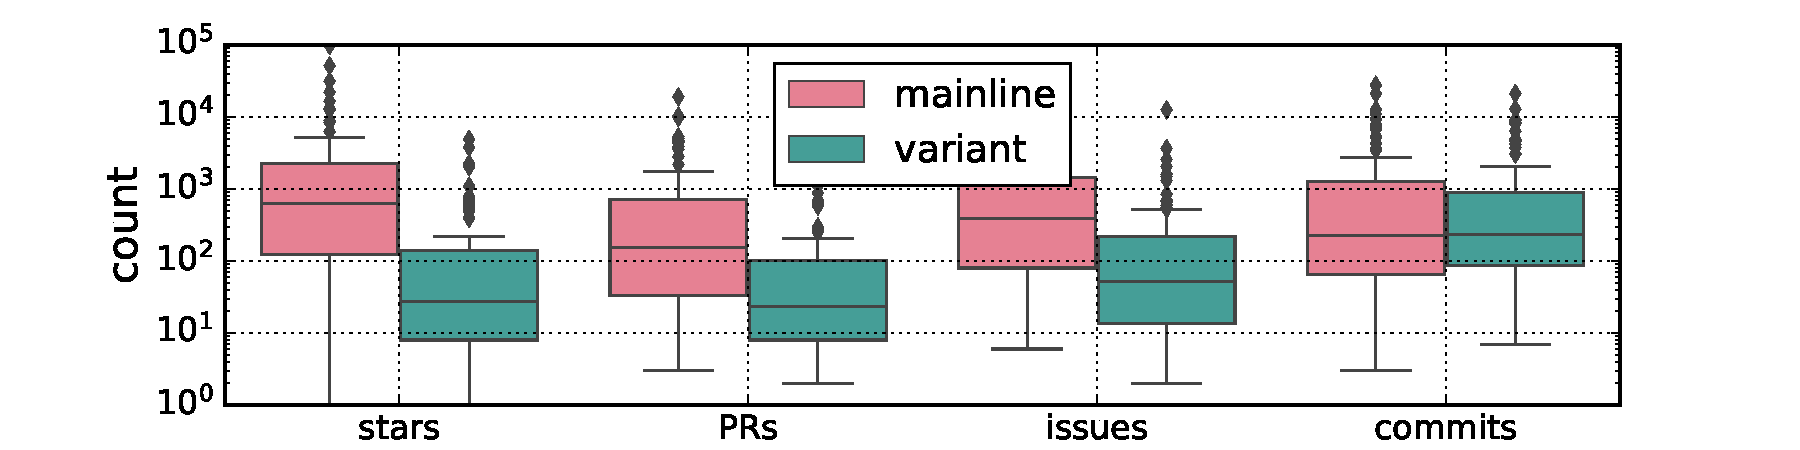
\includegraphics[width=\columnwidth]{pdfs/stats.pdf}
    \caption{Distribution of selected metrics. PRs, issues and commits are counted after the fork date for both mainline and variant.}
    \label{fig:stats}
\end{center}
\vspace{-.3cm}
\end{figure}

In Fig.~\ref{fig:stats} we present the distributions of selected project popularity metrics in of stars, PRs, issues and commits for the 105 mainline--variant pair repositories we investigated. A part from the stars where we consider all in the mainline, we count all (closed + open) PRs, issues, and commits (only main branch) after the fork date. While it is not surprising that the counts for mainline metrics are always higher than those of the variants, it is interesting that most variants are also popular in stars, pull requests and issues counts. This gives us confidence that we are studying real variants as opposed to social forks.
%\ad{I propose to move Fig.~\ref{fig:stats} and the corresponding text to previous section.}

\subsection{Analysis}
\label{sec:card_sorting}
We used card sorting~\cite{zimmermann2016card}, on the 3 open-ended questions which provides a framework to ascertain the meaning and summarize overarching themes of responses within the context of the research question. In the analysis, we grouped similar responses to the open-ended questions into codes. We did not start with any pre-defined codes in mind, but instead derived the codes from the data, iterating as many times as needed until reaching a saturation point. The first iterations of coding was performed by the first author of the paper, and any responses the first author was unsure of were decided by discussion with another author. Once the first two authors agreed on the codes, a virtual meeting was agreed upon where all the other authors joined and discussed the resulting codes and themes and through negotiated agreement~\cite{Garrison:2006}. This approach allowed us to remove duplicates and, in some cases, to generalize or specialize themes, which we will discuss in the later sections of this paper.



